\section{Cluster-based Map Abstraction}
\label{aha:mapabstraction}
The annotated graph we have focused on creating to now is sufficient for a low-level search but inefficient for large problem sizes. 
Instead of planning every step, we would prefer to express a more general strategy using macro-operators.
We will achieve this by starting from the off-line decomposition technique described in \cite{botea04} and extending it to deal with large agents and multiple terrains. 
Our result from theorem {\ref{aha-theorem:reducibility} is key to the spatial abstraction described in this section. 
\par \indent
The general process in \cite{botea04} involves dividing a grid map into \emph{clusters}; subsets of the original grid map which results when the map is divided into a set of fixed-size square sections. Figure \ref{aha-fig:clustersandentrances}(a) shows the result of this decomposition approach; we use clusters of size 5 to split our toy map into 4 adjacent sections.
\par \indent
In the original work \emph{entrances} are obstacle-free transition areas of maximal size which exist along the border area between adjacent pairs of clusters. They are represented in the abstract graph by a pair of nodes connected by an undirected \emph{inter-edge} of weight 1.0. 
Our approach is similar but requires as parameters $C$, the set of all capabilities, and $S$, the set of all agent sizes that will be traversing the map. We thus begin by attempting to identify entrances $\forall c \in C$. Once an entrance is found, we choose as the transition point the first pair of adjacent nodes which maximise clearance. This latter metric is computed by taking the minimum clearance among each node pair in the entrance area and selecting the largest value from the set. The resultant inter-edge $inter$ is annotated such that $inter(c) = cv$. We also impose the following condition:
\begin{equation}
inter(c) > max(s) \Rightarrow inter(c) = max(s) | s \in S
\end{equation}
As we will see in the following section, this truncation step is important for keeping the size of the graph to a minimum.
\par \indent
In figure \ref{aha-fig:clustersandentrances}(b) we present three entrances identified by scanning the border between clusters $c1$ and $c3$.
Entrances \emph{E1} and \emph{E2}, each of which span only part of the border area, are discovered using $\lbrace Ground \rbrace$ and $\lbrace Trees \rbrace$ capabilities. \emph{E3} meanwhile, which spans the whole border area, is discovered using the more complex $\lbrace Ground \vee Trees \rbrace$ capability. 
The connected tiles represent the locations of the subsequent transition points; the final result is shown in \ref{aha-fig:clustersandentrances}(c). 
Note that \emph{E1} and \emph{E3} are incident on the same pair of nodes in the abstract graph. This is due to our  strategy of actively attempting to re-use any existing nodes from the abstract graph. 
We thus produce an abstract \emph{multi-graph}.

\begin{figure}[htbp]
        \caption{\emph{Building clusters and identifying entrances} }
        \begin{center}
                        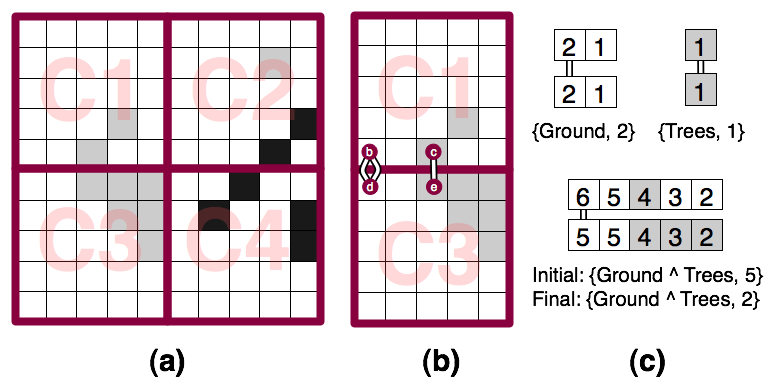
\includegraphics[scale=0.25]{diagrams/identifying_entrances.png}
        \end{center}
        \label{aha-fig:clustersandentrances}
\end{figure}

The final step in the decomposition involves attempting to add to the abstract graph a set of \emph{intra-edges} for each pair of abstract nodes inside a cluster. We achieve this by using AA* such that:
$$ getShortestPath(c, s) \Leftrightarrow intra : c \in C, s \in S $$
\par \indent
Once a path is found we annotate the new edge, $intra$, with the capability and clearance parameters used by AA* and continue the process $\forall (c, s) : c \in C, s \in S$. The algorithm terminates when all clusters have been considered. 
We term the resultant abstraction $initial$ and give the following lemmas to characterise its space complexity:

\input abstractionproperties


To limit the number of inter-edges we add to the abstract graph we will order from lagest to smallest the members of $S$. 
We also order the members of $C$ from simplest (those capabilities containing the least number of terrains) to most complex (the capability corresponding to the set of all terrains). 
\par \indent
The intuition here is that if an inter-edge with large clearance represents the optimal length path between two nodes we would like to re-use it instead of discovering other edges with the same weight and capability using a smaller agent size. This is an instance of edge dominance, a concept we will discuss shortly.
We term the resultant graph a \emph{high-quality abstraction} and present our complete decomposition approach in  algorithm \ref{aha-alg:buildabstraction}.
\par \indent
The result of this approach is highlighted in figure \ref{aha-fig:abstractgraph}(a), where we show the 13 identified intra-edges and their annotations for the pair of clusters from the previous example. In figure \ref{aha-fig:abstractgraph}(c) we can see the complete graph for our running example; we were able to represent a 2-terrain map with 100 nodes and 350 edges using just 13 nodes and  23 edges. 

\input algorithms/alg_buildabstraction

\subsection{Optimising Abstract Graph Size}
A possible risk with our decomposition algorithm is that as the number of terrains in the environment increase the size of the abstract graph will become larger and larger and in turn, result in greater memory usage and decreased planning performance as our agent has to evaluate a greater number of possible routes.
One strategy for addressing this problem is to use the concept of weak dominance relationships to minimise the number of edges we add to the abstract graph. 

\begin{definition}
A \emph{dominance relationship} is said to exist between two annotated edges when both cover the same pair of nodes but one represents a wider corridor which is traversable using the capability of the other. If the dominant edge has a shorter traversal cost, the relationship is said to be strongly dominant. Otherwise, the dominance is weak.
\end{definition}

The idea is simple: if two nodes are connected by multiple edges with overlapping traversal requirements we prefer to keep the edge with the largest clearance and most general capability (ie. involving fewer terrains), irrespective of comparative differences in length. A reasonable analogy we could draw at this point is to compare the way off-road vehicles opportunistically use roads where possible even if an off-road route (or trail) might exist which has a smaller distance cost. We prefer roads because are smoother to drive on and have other benefits such less wear and tear, better fuel consumption per kilometer ratio and so on. Of course, opting for a lower-quality abstraction in this way does have an effect on the quality of the computed solutions, but as we will show in our experimental analysis, the differences are reasonably small and the solutions still near-optimal for our test data. The best choice here depends on the requirements of the specific application to which the algorithm is applied; it is a classic tradeoff between performance vs space.

In \ref{aha-fig:abstractgraph}d we show a low-quality abstraction. In this trival example we could only reduce the abstract edge count by 2 (in cluster \emph{C1}) but this is an atypical result as we will later demonstrate.

\begin{figure}[htbp]
        \caption{\emph{High and low quality abstraction results} }
        \begin{center}
                        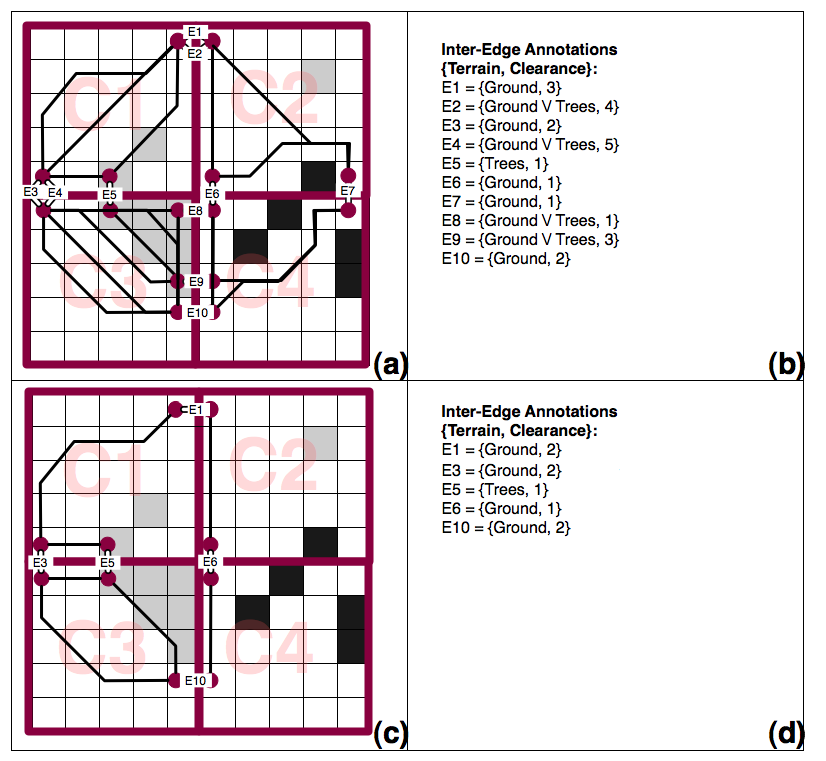
\includegraphics[scale=0.25]{diagrams/abstraction_result.png}
        \end{center}
        \label{aha-fig:abstractgraph}
\end{figure}
